\section{Introduction}

\todo{Remember to use anonymous submission}The ability for neurons to hold numbers and do arithmetic operations has been documented in both humans, non-human primates \cite{nieder-neuronal-number}, newborn chicks \cite{rugani-arithmetic-chicks} and bees \cite{gallistel-numbers-in-brain}.
In our quest to solve intelligence we have put much faith in neural networks, which in turn has provided unparalleled and often superhuman performance in many tasks requiring high cognitive ability \cite{natureGo,googleNMT,resnet}.
However, when using neural networks to solve simple arithmetic problems, such as counting, they systematically fail to extrapolate \cite{stillNotSystematic,suzgun2019evaluating,trask-nalu}. \todo{Extend. Not convincing enough.}

In this paper, we analyze and improve parts of the recently proposed Neural Arithmetic Logic Unit (NALU) \cite{trask-nalu}. Our contribution is an alternative formulation of the weight constraint with a clipped linear activation, a regularizer that bias towards sparse solutions, and a reformulation of the multiplication unit to be partially linear. All of which significantly improves upon the existing $\text{NAC}_{+}$ and $\text{NAC}_{\bullet}$ units as shown through extensive testing on arithmetic constructions.% \footnote{In the interest of scientific integrity, we have made the code for all experiments, and more, available on GitHub: \censor{\url{https://github.com/AndreasMadsen/stable-nalu}}.}

\begin{figure}[h]
\centering
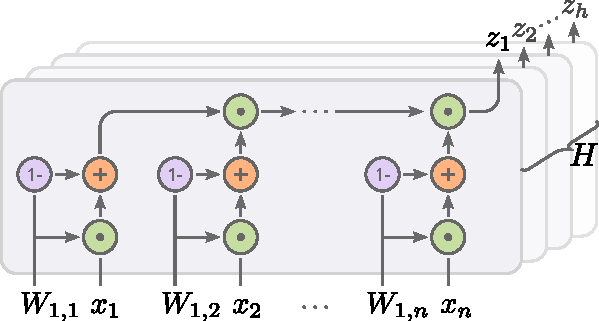
\includegraphics[scale=0.8]{graphics/nmu.pdf}
\caption{Visualization of NMU for a single output scalar $z_1$, this construction repeats for every element in the output vector $\mathbf{z}$.}
\end{figure}

The NALU is a neural network layer with two sub-units. The two sub-units, $\text{NAC}_{+}$ for addition/subtraction and $\text{NAC}_{\bullet}$ for multiplication/division, are softly gated between with a sigmoid function. By using trainable weights, and restricting the weights towards $\{-1,0,1\}$. The weights are learned by observing arithmetic input-output pairs and using backpropagation\cite{rumelhart1986learning}. \todo{1. restricting and towards are in opposition. 2. Difficult to understand without knowing NALU.}

We focus only on the $\text{NAC}_{+}$ and $\text{NAC}_{\bullet}$ as we have found that the gating in NALU can be cumbersome, as shown in table \ref{tab:function-task-static-defaults} where the NALU performs significantly worse than $\text{NAC}_{+}$ and $\text{NAC}_{\bullet}$. This is because of the difficulties in selecting between, and simultaneously training, two vastly different operations.

We will thus assume that the appropriate operation is already known, or can empirically be found by varying the network architecture (oracle gating). We find that the $\text{NAC}_{+}$ and $\text{NAC}_{\bullet}$ units poses optimization difficulties. We present the following findings: \todo{Reduce space?}

\begin{itemize}
\item The gradients from the weight matrix construction in $\text{NAC}_{+}$ and $\text{NAC}_{\bullet}$, have zero expectation.

\item The $\text{NAC}_{\bullet}$ have a treacherous optimization space with unwanted global minimas (as shown in figure \ref{fig:nac-mul-eps-issue}) and have exploding/vanishing gradients.

\item Using the addition module $\text{NAC}_{+}$, we observe that the wanted weight matrix values of $\{-1, 0, 1\}$ is rarely found.
\end{itemize}

Motivated by these convergence and sparsity issue, we propose alternative formulations of the $\text{NAC}_{+}$ and $\text{NAC}_{\bullet}$, which we call the Neural Addition Unit (NAU) and Neural Multiplication Unit (NMU).

%It is fair to assume that the ability to perform arithmetic operations is crucial modern intelligence.
%However, Neural networks(nature, yann lecun), even though it has great expressiveness, has shown an inability to count severe lacks the ability to explicitly only has the ability to has an extreme capacity to interpolate complex functions from simply observing data (ICLR best paper 2017).
%However, even when extrapolating to unseen data we often find a sharp in performance.\cite{missing-cite:image-with-modification}(systematic, nalu, Anders paper).
%Such inability to extrapolate either requires the training distribution to cover the entire distribution (DAGGER) or simply restrics certain systems to be built all together.

%Our solution

%Experiments

%Results





%Remove
%So far, there have not been much research in training exact arithmetic operations for extrapolation. The most important research, is by far, the recently proposed NAC and NALU \cite{trask-nalu}. However, as we will show both analytically and empirically, their results are highly exaggerated, as the proposed arithmetic units are extremely difficult to make convergence consistently. In fact, even without gating mechanism their multiplication operator can't converge on extremely simple problems. For the cases of addition there do converge, a nearly sparse weight matrix of values close to ${-1, 0, 1}$ is rarely found, which also contradicts one of their core claims.
%Motivated by these convergence and sparsity issue, we focus on improving the arithmetic units themself, without considering the gating mechanism in NALU. That is, we will assume that the appropriate operation is already known, or can empirically be found by varying the network architecture which is very common when developing neural networks.